\documentclass{scrartcl}

\usepackage{tikz}
\usetikzlibrary{calc}						%for centerarc
\usetikzlibrary{decorations.pathmorphing}	%for random drapery	

\def\centerarc[#1](#2)(#3:#4:#5)% Syntax: [draw options] (center) (initial angle:final angle:radius)
{ \draw[#1] ($(#2)+({#5*cos(#3)},{#5*sin(#3)})$) arc (#3:#4:#5); }

%from Deleuze - The Fold: Leibniz and the Baroque (1993), p. 5
%this paper gives a comparison between the original & the one in the English translation
%https://altexploit.files.wordpress.com/2017/05/diagrams-as-piloting-devices-deleuze.pdf

%note: the drapery uses random numbers, so it changes when anything else in the file is changed

\begin{document}
	
	\hspace{-2.5cm}
	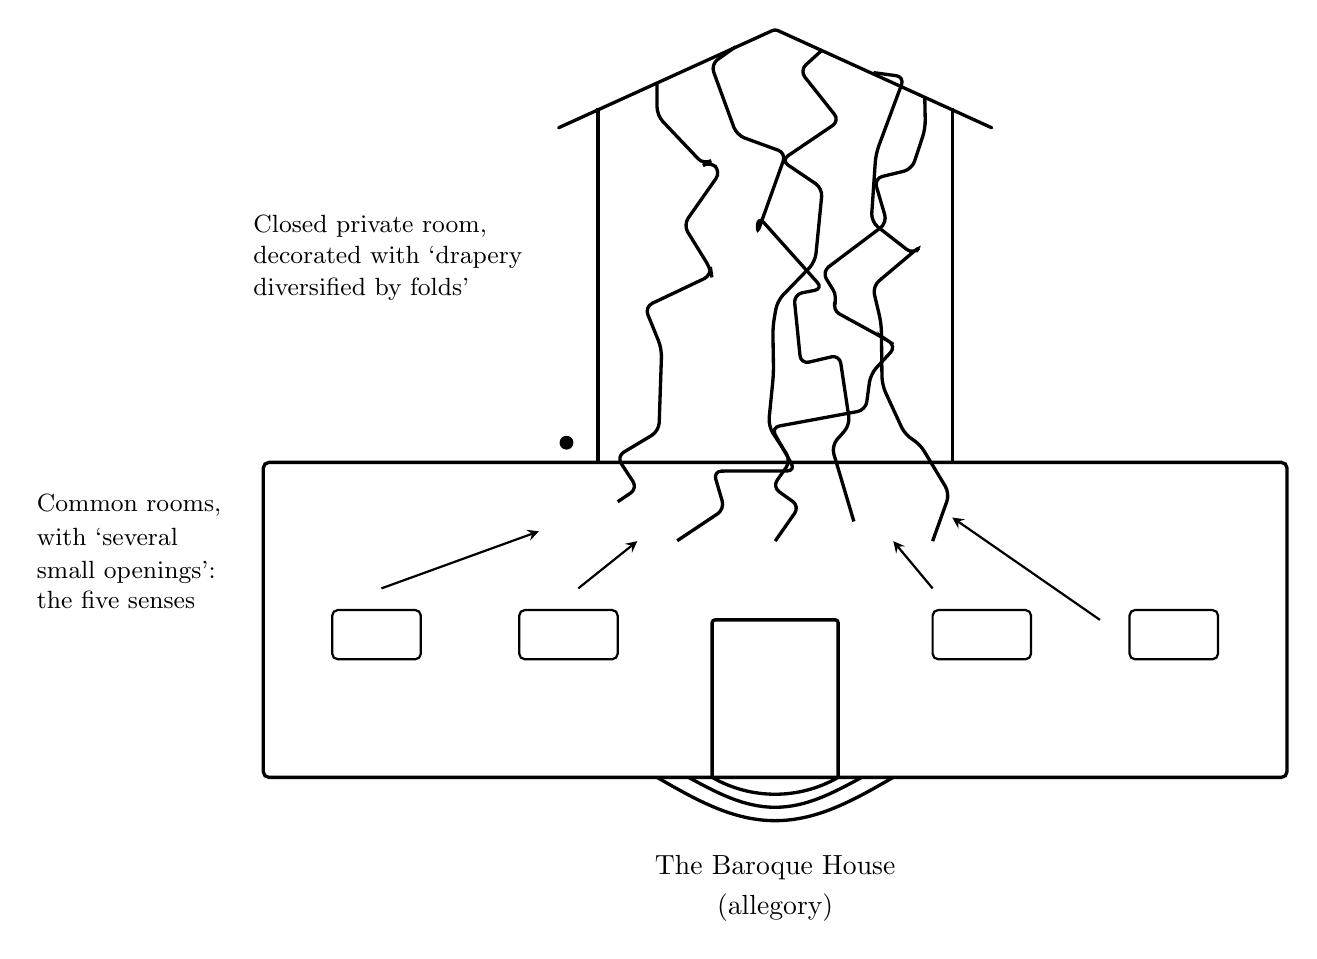
\begin{tikzpicture}
	%HOUSE	
	\draw[very thick,rounded corners=1pt,line cap=round] (2.75,8.25)--(0,9.5)--(-2.75,8.25);
	\draw[very thick] (-2.25,4)--(-2.25,8.5);	%steeple walls
	\draw[very thick] ( 2.25,4)--( 2.25,8.5);
	%
	\draw[thick,rounded corners=2pt] (-3.25,1.5) rectangle (-2,2.125);		%windows
	\draw[thick,rounded corners=2pt] (-4.5, 1.5) rectangle (-5.625,2.125);
	\draw[thick,rounded corners=2pt] ( 4.5, 1.5) rectangle ( 5.625,2.125);
	\draw[thick,rounded corners=2pt] ( 3.25,1.5) rectangle ( 2,2.125);
	%
	\draw[thick,->,>=stealth] (-5,2.4)--(-3,3.125);
	\draw[thick,->,>=stealth] (-2.5,2.4)--(-1.75,3);
	\draw[thick,->,>=stealth] (2,2.4)--(1.5,3);
	\draw[thick,->,>=stealth] (4.125,2)--(2.25,3.3);
	%
	\draw[very thick,rounded corners=2pt] (-6.5,0) rectangle (6.5,4);	%house
	\draw[very thick,rounded corners=1pt] (-0.8,0)--(-0.8,2)--(0.8,2)--(0.8,0);	%door
	\draw[very thick] (-0.8,0) arc (240:300:1.6);
	\draw[very thick] (-1.1,0) sin (0,-0.38) cos (1.1,0);
	\draw[very thick] (-1.5,0) sin (0,-0.55) cos (1.5,0);
	
	%DRAPERY
	\draw[very thick,decorate,decoration={random steps,segment length=0.5cm,amplitude=4mm},rounded corners=3pt] (-1.5,8.83)--(-1.5,8.5)--(-0.75,7.75)--(-2,3.5);
	\draw[very thick,decorate,decoration={random steps,segment length=0.5cm,amplitude=4mm},rounded corners=3pt] (-0.5,9.28)--(1,3.25);
	\draw[very thick,decorate,decoration={random steps,segment length=0.5cm,amplitude=4mm},rounded corners=3pt] ( 0.6,9.24)--(0,3);
	\draw[very thick,decorate,decoration={random steps,segment length=0.5cm,amplitude=4mm},rounded corners=3pt] (1.25,8.95)--(2,3);
	\draw[very thick,decorate,decoration={random steps,segment length=0.5cm,amplitude=4mm},rounded corners=3pt] (1.9,8.65)--(0.75,6)--(1.5,5.5)--(-1.25,3);
	
	%DECORATION AT LEFT CORNER
	\fill (-2.65,4.25) circle (2.5pt);
	\centerarc[very thick,line cap=round](-2.65,4.25)(315:60:0.25)
	\centerarc[very thick](-2.45,4.65)(-110:90:0.2)
	\centerarc[very thick,line cap=round](-2.45,4.75)(90:270:0.1)
	
	%CAPTIONS
	\node[align=left,right] at (-6.75,7.0) {\small Closed private room,};
	\node[align=left,right] at (-6.75,6.6) {\small decorated with `drapery};
	\node[align=left,right] at (-6.75,6.2) {\small diversified by folds'};
	%
	\node[align=left,right] at (-9.5,3.45) {\small Common rooms,};
	\node[align=left,right] at (-9.5,3.05) {\small with `several};
	\node[align=left,right] at (-9.5,2.60) {\small small openings':};
	\node[align=left,right] at (-9.5,2.25) {\small the five senses};
	%
	\node at (0,-1.15) {The Baroque House};
	\node at (0,-1.65) {(allegory)};
	\end{tikzpicture}
	
\end{document}